\section{Experimentación y resultados}

\subsection{Resultados globales}

La Tabla 2 resume los resultados agregados sobre los 32 comandos del
dataset. Los cuatro modelos alcanzaron 100\% de validez de formato JSON, lo
que indica que incluso el modelo más pequeño (360M parámetros) es capaz de
seguir instrucciones de formato estructurado de forma consistente en este
dominio acotado.

\begin{table}[htbp]
\centering
\caption{Resultados globales por modelo (n=32 comandos).}
\label{tab:orig-globales}
\begin{tabular}{lllll}
\toprule
Modelo & Parámetros & JSON válido & Coincidencia exacta & Latencia (s) \\
\midrule
SmolLM2-360M & 0.36B  & 100.0\% & 18.8\% & 15.6 \\
Qwen2.5-0.5B & 0.494B & 100.0\% & 43.8\% & 14.7 \\
Qwen2.5-1.5B & 1.54B  & 100.0\% & 50.0\% & 43.2 \\
SmolLM2-1.7B & 1.71B  & 100.0\% & 59.4\% & 61.9 \\
\bottomrule
\end{tabular}
\end{table}

\begin{figure}[htbp]
\centering
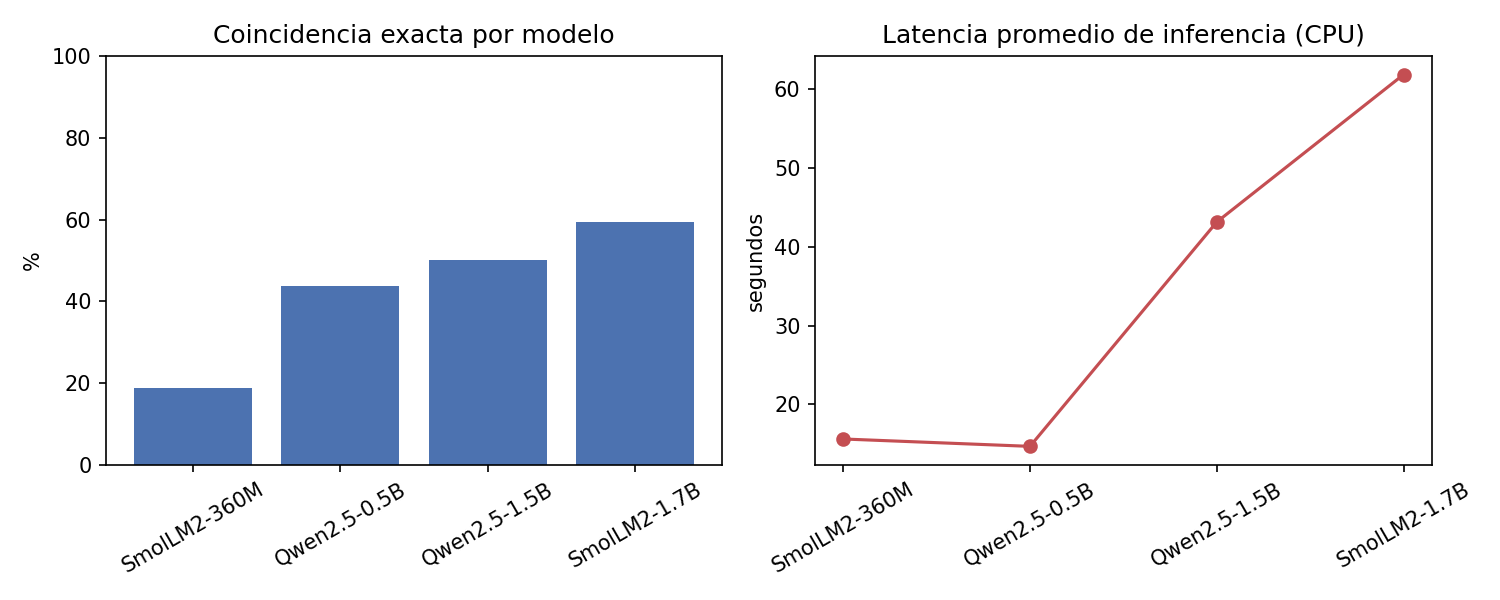
\includegraphics[width=\textwidth]{../../figures/fig1_exactitud_latencia.png}
\caption{Coincidencia exacta (izquierda) y latencia promedio de inferencia en
CPU (derecha), por modelo.}
\label{fig:orig-fig1}
\end{figure}

La coincidencia exacta crece de forma consistente con el tamaño del modelo
(18,8\% → 43,8\% → 50,0\% → 59,4\%), pero la latencia crece de forma mucho
más pronunciada: el modelo más grande (SmolLM2-1.7B) es casi 4 veces más
lento que el más chico (61,9s vs. 15,6s por comando), y llamativamente más
lento que Qwen2.5-1.5B (43,2s) a pesar de tener un 11\% más de parámetros —
una diferencia que probablemente responda a diferencias arquitectónicas o
de tokenizador entre familias, y no únicamente al conteo de parámetros.

\subsection{Exactitud por campo del esquema}

Descomponer la exactitud por campo (Fig. 2) muestra un patrón más matizado
que el de la coincidencia exacta agregada. Los campos intent, dispositivo y
ubicación mejoran de forma clara con el tamaño del modelo (intent: 40,6\% →
84,4\% → 93,8\% → 87,5\%; ubicación: 71,9\% → 81,2\% → 90,6\% → 96,9\%). En
cambio, los campos valor y unidad se mantienen relativamente estancados
entre 75\% y 90\% en los cuatro modelos, sin una tendencia monótona clara —
el modelo más grande (SmolLM2-1.7B) no supera a Qwen2.5-1.5B en ninguno de
estos dos campos.

\begin{figure}[htbp]
\centering
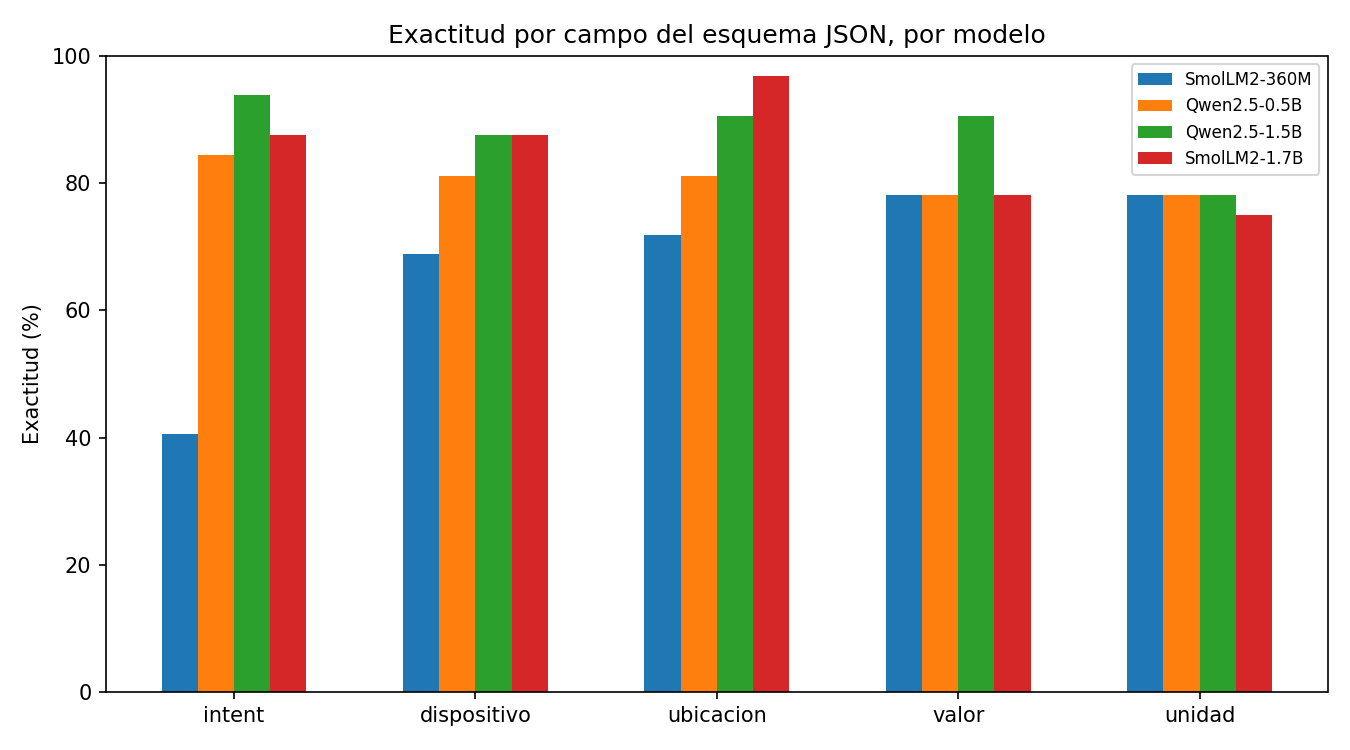
\includegraphics[width=\textwidth]{../../figures/fig2_exactitud_por_campo.png}
\caption{Exactitud por campo del esquema JSON (intención, dispositivo,
ubicación, valor, unidad), por modelo.}
\label{fig:orig-fig2}
\end{figure}

\subsection{Exactitud por categoría de comando}

La Tabla 3 desagrega la coincidencia exacta por categoría lingüística. Las
columnas de modelo se abrevian por su cantidad de parámetros (360M, 0.5B,
1.5B, 1.7B), en el mismo orden que la Tabla 2. La categoría de ajustes
relativos o cualitativos sin valor numérico explícito (por ejemplo,
``bajale un poco a la luz del living'') es, por lejos, la más difícil para
los cuatro modelos, con una exactitud de apenas 0\% a 16,7\% incluso en el
modelo más grande evaluado. Es importante notar que las categorías de
consulta de estado y negación/contexto tienen sólo 3 comandos cada una, por
lo que sus porcentajes deben leerse con cautela (representan 1 o 2 aciertos
sobre 3 casos).

\begin{table}[htbp]
\centering
\caption{Coincidencia exacta por categoría lingüística de comando y modelo.}
\label{tab:orig-categorias}
\begin{tabular}{lllll}
\toprule
Categoría (n) & 360M & 0.5B & 1.5B & 1.7B \\
\midrule
Encendido / apagado simple (n=8)           & 12.5\% & 62.5\% & 62.5\% & 75.0\% \\
Ajuste con valor numérico (n=8)            & 25.0\% & 75.0\% & 87.5\% & 87.5\% \\
Ajuste relativo / cualitativo (n=6)        & 0.0\%  & 0.0\%  & 16.7\% & 16.7\% \\
Múltiples dispositivos (n=4)               & 0.0\%  & 25.0\% & 25.0\% & 50.0\% \\
Consulta de estado (n=3)                   & 66.7\% & 33.3\% & 33.3\% & 33.3\% \\
Negación / contexto conversacional (n=3)   & 33.3\% & 33.3\% & 33.3\% & 66.7\% \\
\bottomrule
\end{tabular}
\end{table}

\subsection{Análisis cualitativo de errores}

Para caracterizar mejor la naturaleza de los errores más allá del
porcentaje agregado, se clasificó manualmente cada una de las 73 respuestas
incorrectas (sobre 128 corridas totales) en una o más de cuatro categorías
no excluyentes: confusión de intención (el campo intent no coincide),
confusión de dispositivo, confusión de ubicación, y alucinación de
valor/unidad (el modelo asigna un valor o unidad numérica cuando el ground
truth es null) o valor numérico incorrecto (cuando sí correspondía un
número pero el valor difiere). La Tabla 4 resume esta clasificación.

\begin{table}[htbp]
\centering
\caption{Taxonomía de errores por modelo (cantidad de casos por categoría,
sobre el total de respuestas incorrectas de cada modelo; un caso puede
pertenecer a más de una categoría).}
\label{tab:orig-taxonomia}
\begin{tabular}{lllll}
\toprule
Categoría de error & 360M & 0.5B & 1.5B & 1.7B \\
\midrule
Total de respuestas incorrectas & 26 & 18 & 16 & 13 \\
Confusión de intención          & 19 & 5  & 2  & 4  \\
Confusión de dispositivo        & 10 & 6  & 4  & 4  \\
Confusión de ubicación          & 9  & 6  & 3  & 1  \\
Alucinación de valor/unidad     & 0  & 5  & 7  & 7  \\
Valor numérico incorrecto       & 7  & 2  & 1  & 1  \\
\bottomrule
\end{tabular}
\end{table}

La taxonomía revela un desplazamiento cualitativo del error dominante a
medida que crece el modelo: en SmolLM2-360M, el 73\% de los errores (19 de
26) son confusión de intención, mientras que la alucinación de valor/unidad
es inexistente en ese modelo. En SmolLM2-1.7B ocurre lo opuesto: la
confusión de intención cae a 4 casos pero la alucinación de valor/unidad
pasa a ser, junto con la confusión de dispositivo, el error más frecuente
(7 de 13, 54\%) — consistente con la Sección 4.2: los modelos grandes
aprenden mejor qué intención y dispositivo corresponden, pero no a
abstenerse de completar un valor inexistente.

Un ejemplo particularmente ilustrativo es el comando ``Hace un poco más de
calor en el dormitorio, subí la calefacción'' (ground truth: valor=null,
unidad=null): SmolLM2-360M-Instruct confundió directamente la intención
(predijo ``consultar'' en lugar de ``ajustar''); Qwen2.5-0.5B-Instruct
predijo valor=15, unidad=``\%''; Qwen2.5-1.5B-Instruct predijo
unidad=``$^{\circ}$C'' (sin valor); y SmolLM2-1.7B-Instruct predijo valor=2,
unidad=``$^{\circ}$C''. Los cuatro modelos fallaron, pero de maneras
cualitativamente distintas — el más chico por no entender la intención, los
tres restantes por alucinar una cifra o unidad inexistente en el comando
original.

Un segundo hallazgo surgió al inspeccionar los errores de ``confusión de
dispositivo'': varios no son errores semánticos sino de vocabulario. Ante el
comando ``Che, la tele del living quedó prendida, apagala por favor''
(ground truth: dispositivo=``tv''), los cuatro modelos identificaron
correctamente intención, ubicación y ausencia de valor, pero usaron
sinónimos distintos: SmolLM2-360M y Qwen2.5-0.5B predijeron ``tele'',
Qwen2.5-1.5B predijo ``televisor'', y ninguno usó el token ``tv'' del
vocabulario del prompt. Bajo coincidencia exacta estos casos se contabilizan
como error, aunque semánticamente la interpretación es correcta — un punto
retomado como amenaza a la validez de constructo en la Sección 6.
